\documentclass[a4paper,12pt]{article}
\usepackage[utf8]{inputenc}
\usepackage{graphicx}
\usepackage{subcaption}
\usepackage{amsmath}
\usepackage{url}
\usepackage{float}
\usepackage{babel}
\renewcommand{\figurename}{Slika}  % Change "Figure" to "Slika"
\renewcommand{\tablename}{Tabela}

\begin{document}

\begin{titlepage}
    \centering
	\begin{figure}[htbp]
    	\centering
    	
\includegraphics[width=0.4\textwidth]{./logo.png}
	\end{figure}
    { Univerzitet u Beogradu \\ Matematički fakultet\par}
	
    \vfill

    {\Large \textbf{Seminarski rad}\par}

    \vspace{1cm}

    {\Large \textbf{Ocenjivanje broja ljudi na javnom skupu}\par}

    \vfill

    
	
	
	\begin{tabbing}
	\hspace{10cm} \= \hspace{10cm} \= \kill
	\textbf{Mentor:} \>  \textbf{Studenti:} \\
	dr Marija Cuparić \> Lana Matić 143/2021 \\
	Luka Perović \> Anja Milutinović 235/2021 \\
	\> Smer: Informatika
	\end{tabbing}

    \vfill

    \textbf{Datum:} 2024/25

\end{titlepage}
\newpage
\tableofcontents
\newpage
\section{Uvod}

Procena broja ljudi na javnim skupovima važna je za bezbednost, logistiku, planiranje resursa i evaluaciju događaja. Tradicionalne metode brojanja na terenu često su skupe, spore i podložne greškama, naročito kada je gužva neujednačena i kada uslovi posmatranja variraju između lokacija.
Cilj ovog rada je procena ukupnog broja ljudi prisutnih na Slaviji 15.3.2025. , na osnovu slika dobijenih iz drona. 
\newline
\newline
\noindent Korisitićemo stratifikovano uzorkovanje nad slikama podeljenim mrežom sa automatskim razvrstavanjem ćelija u stratume po gustini, kako bi se efikasno i transparentno ocenili ukupan broj prisutnih ljudi.
Polazni skup podataka čine fotografije dobijene izdvajenjem frejmova iz video-snimka dronom, dalje isečenih u sedam međusobno disjunktnih slika koje pokrivaju različite ulice posmatranog područja.
Koristimo stratifikovano uzorkovanje sa pilot fazom i Neymanov metod raspodele obima uzorka po stratumima.
\newline
\newline
\noindent Rezultati su primenljivi u realnim uslovima i lako se prilagođavaju drugim lokacijama, rezolucijama i opterećenjima scene.
\newline
\newline
\noindent Napomena da metod ima ograničenja, jer tačnost zavisi od kvaliteta ulaznih snimaka (osvetljenje, senke, refleksije, zaklanjanja), kao i od stabilnosti veze između vizuelnih signala i stvarne prisutnosti ljudi.




\newpage
\section{Prikupljanje materijala}

Materijali korišćeni u radu prikupljeni su pomoću snimka dobijenog iz drona \cite{drone_video}, izdvajanjem određenih frejmova koji odgovaraju različitim ulicama. Slike su zatim dodatno isečene tako da nema značajnih preklapanja, radi izbegavanja pojavljivanja istih delova na različitim slikama.
Na narednim slikama prikazani su frejmovi izdvojeni iz snimka dronom.

\begin{figure}[H] 
	\centering 
	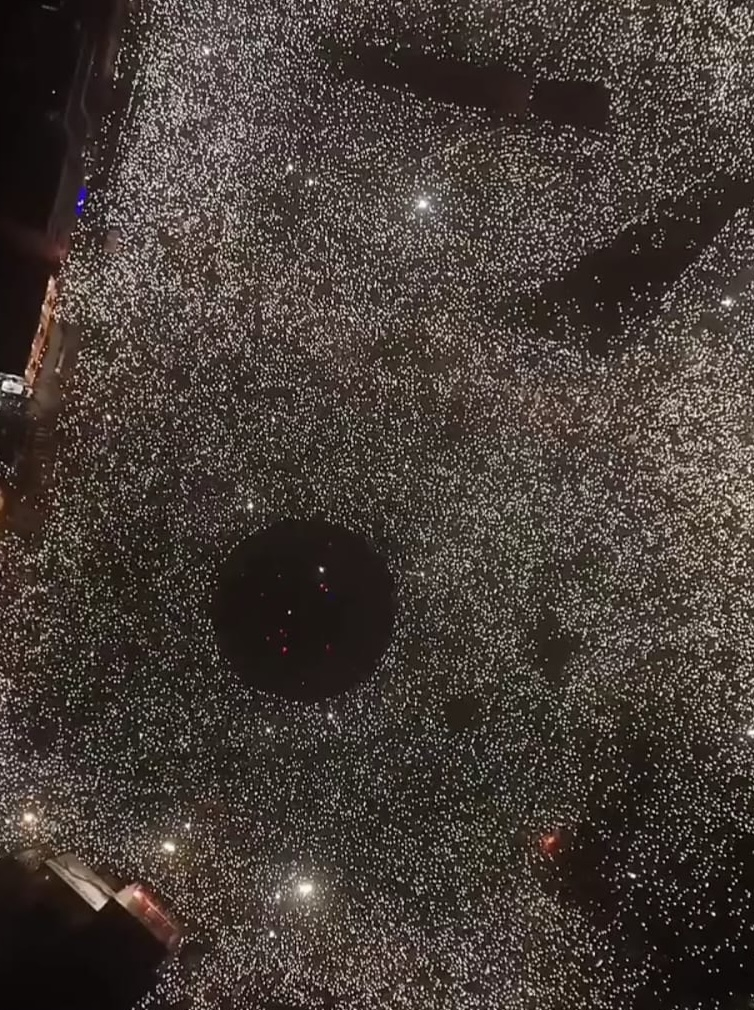
\includegraphics[width=0.8\textwidth]{../images/slavija-centar.jpeg} 
	\caption{Slavija.} 
	\label{fig:slavija} 
\end{figure}

\begin{figure}[H]
	\centering
  
	% Prvi red
	\begin{subfigure}[b]{0.3\textwidth}
	  \centering
	  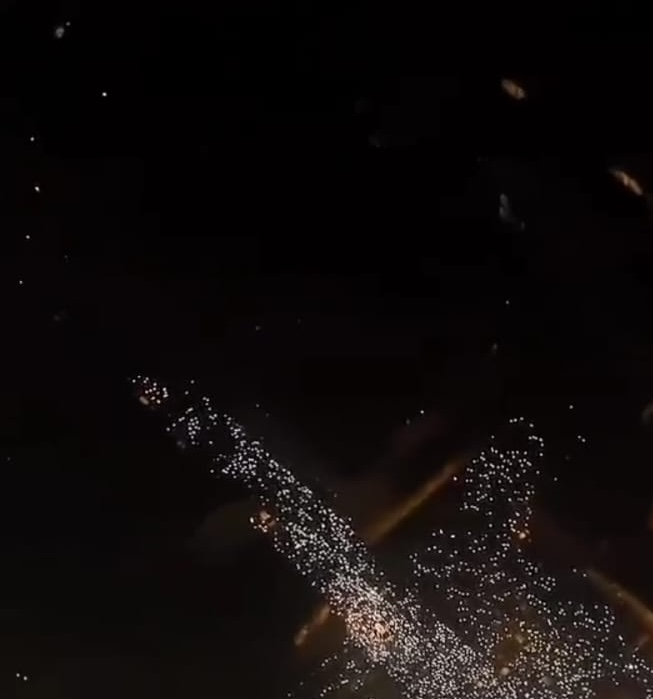
\includegraphics[width=\textwidth]{../images/prote-mateje.jpeg}
	  \caption{Prote Mateje}
	  \label{fig:prote-mateje}
	\end{subfigure}
	\hfill
	\begin{subfigure}[b]{0.3\textwidth}
	  \centering
	  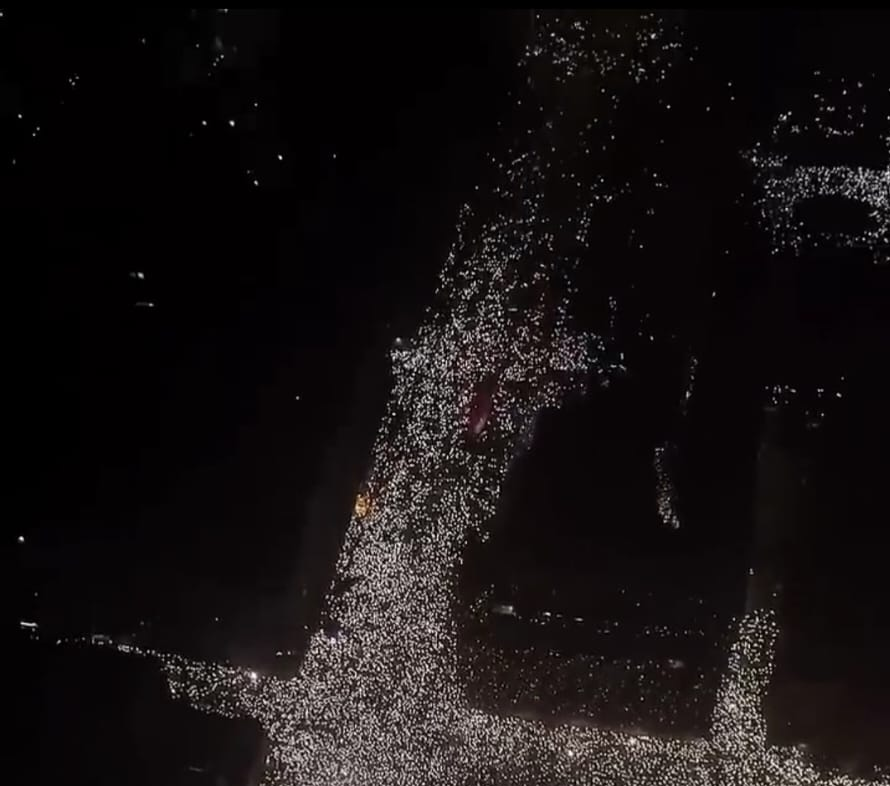
\includegraphics[width=\textwidth]{../images/nemanjina.jpeg}
	  \caption{Nemanjina}
	  \label{fig:nemanjina}
	\end{subfigure}
	\hfill
	\begin{subfigure}[b]{0.3\textwidth}
		\centering
		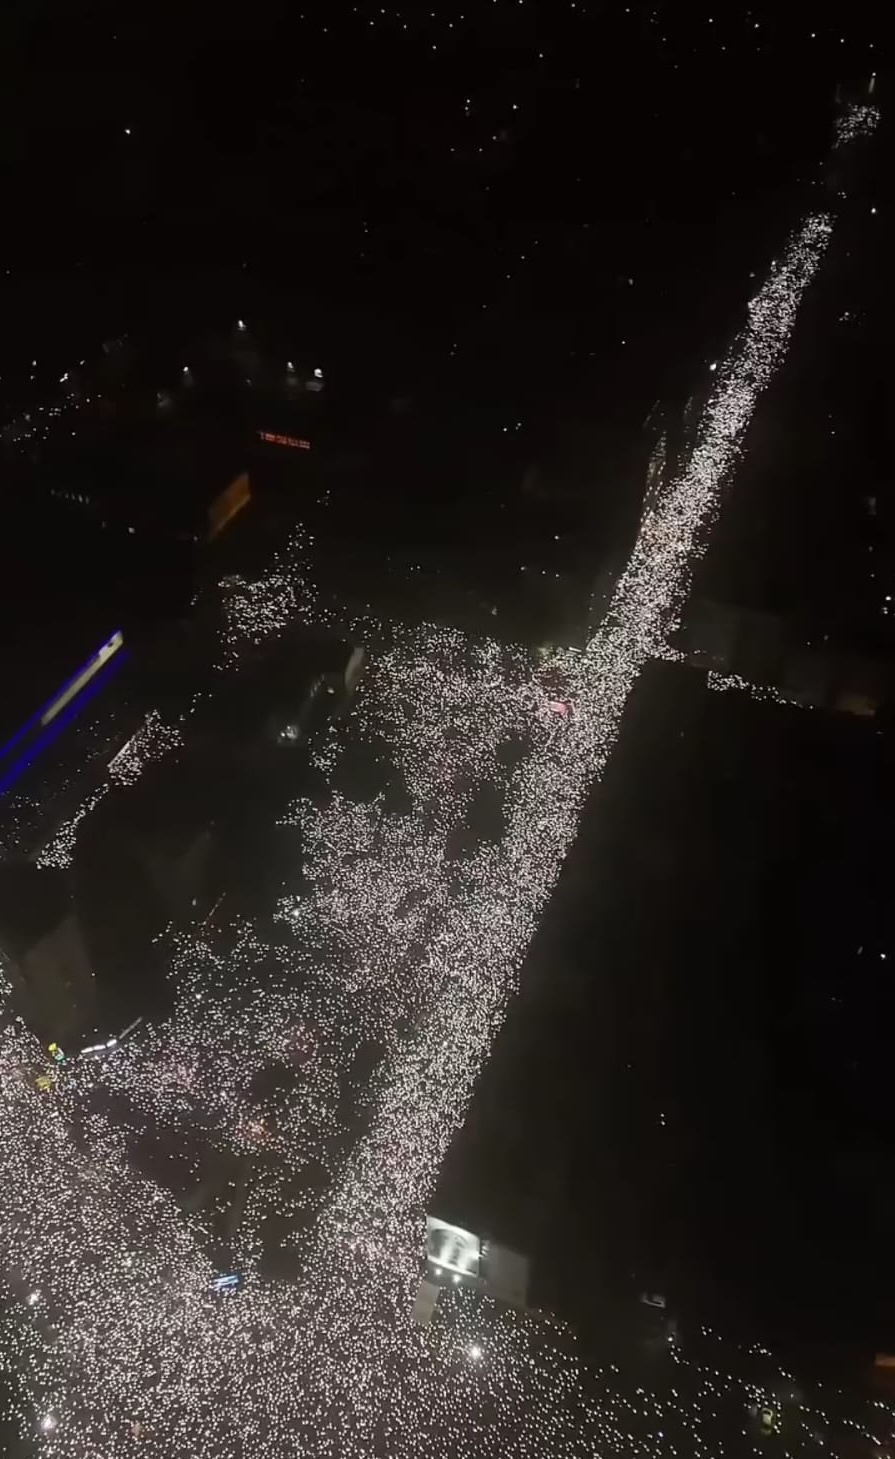
\includegraphics[width=\textwidth]{../images/beogradska.jpeg}
		\caption{Beogradska}
		\label{fig:beogradska}
	\end{subfigure}
  
	\vspace{0.3cm} % razmak između redova
  
	% Drugi red
	\begin{subfigure}[b]{0.3\textwidth}
	  \centering
	  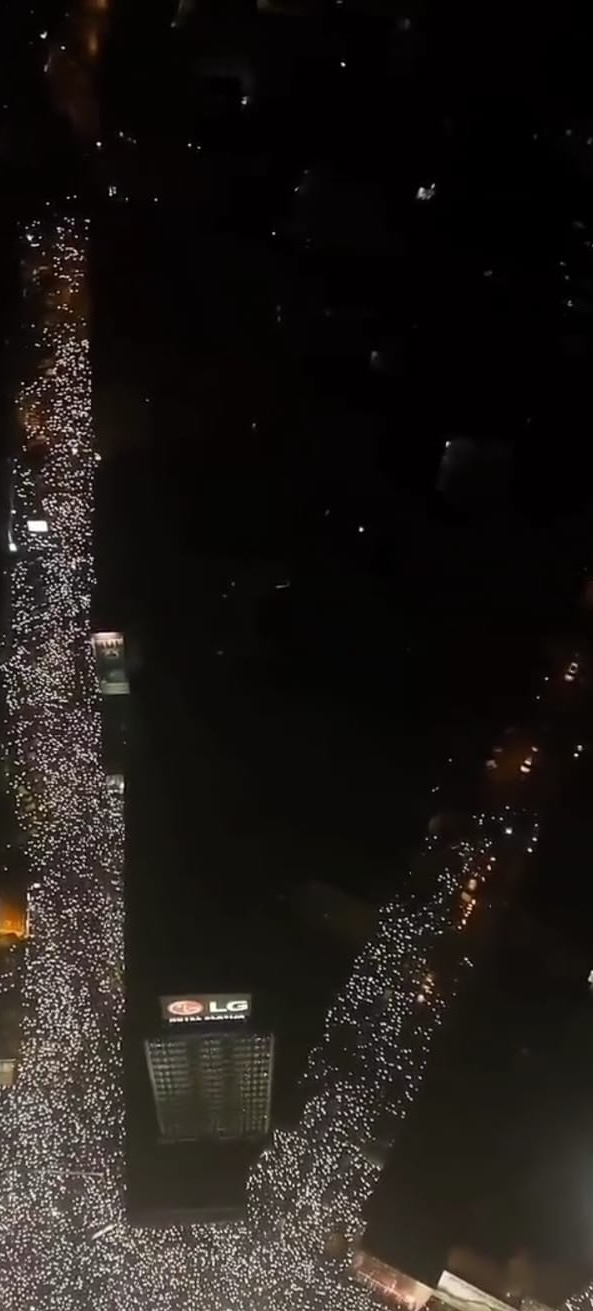
\includegraphics[width=\textwidth]{../images/makenzijeva.jpeg}
	  \caption{Makenzijeva}
	  \label{fig:makenzijeva}
	\end{subfigure}
	\hfill
	\begin{subfigure}[b]{0.3\textwidth}
	  \centering
	  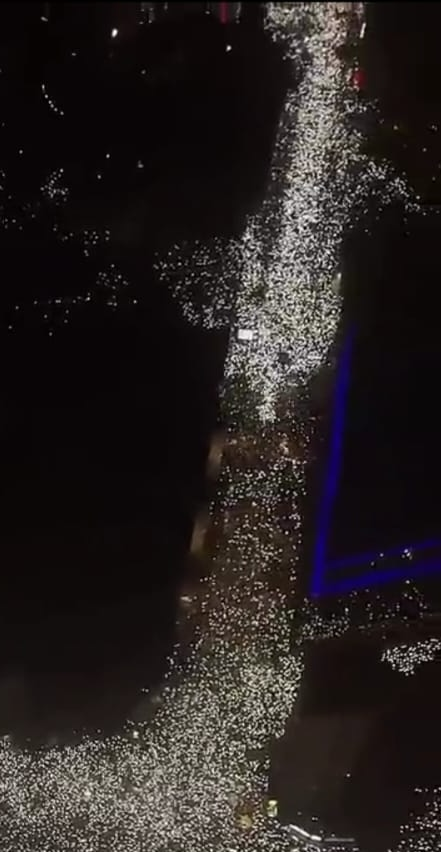
\includegraphics[width=\textwidth]{../images/kralja-milana.jpeg}
	  \caption{Kralja Milana}
	  \label{fig:kralja-milana}
	\end{subfigure}
	\hfill
	\begin{subfigure}[b]{0.3\textwidth}
	  \centering
	  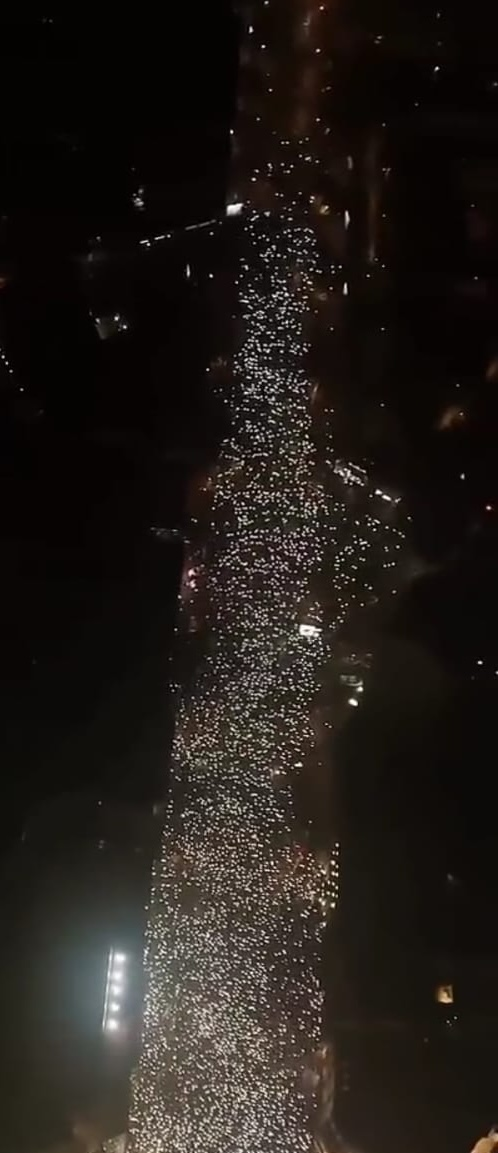
\includegraphics[width=\textwidth]{../images/bulevar-oslobodjenja.jpeg}
	  \caption{Bulevar oslobođenja}
	  \label{fig:bulevar-oslobodjenja}
	\end{subfigure}
  
	\caption{Pregled ulica sa snimka dronom}
\end{figure}

\newpage
\section{Grid i stratifikacija}

Kako bi se omogućili uzorkovanje, svaka ulazna slika je podeljena na pravougaoni grid dimenzija 40 x 40 ćelija. 
Mreža je naprvaljena u R-u, i za svaku ćeliju su čuvani sledeći atributi: 
jedinstveni identifikator - \texttt{cell\_id}, red i kolonu, koordinate u pikeslima \texttt{(x0, x1, y0, y1)}, oznaku zone - \texttt{zone\_id}, 
logičku oznaku - \texttt{include} - da li je ćelija uključena u uzorkovanje i stratumski indeks - stratum.
Informacije čuvamo u tabeli \texttt{starta\_map.csv}, koju zatim popunjavamo.

\begin{figure}[H] 
	\centering 
	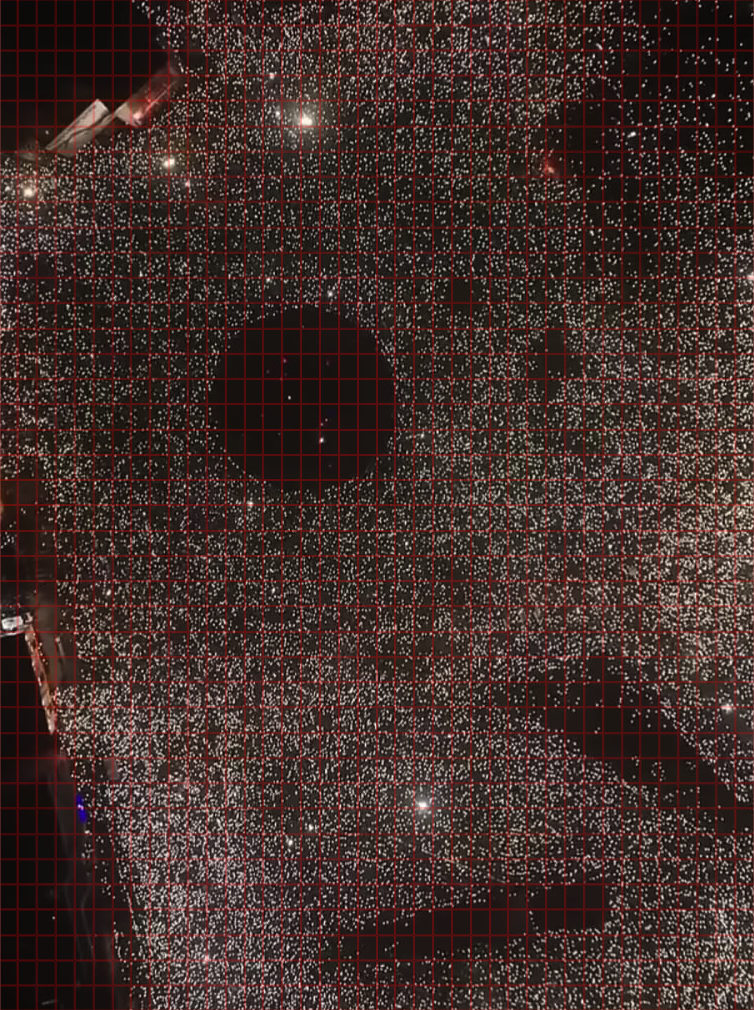
\includegraphics[width=0.8\textwidth]{../grid_output/slavija-centar_grid.png} 
	\caption{Slavija.} 
	\label{fig:slavija} 
\end{figure}

\begin{figure}[H]
	\centering
  
	% Prvi red
	\begin{subfigure}[b]{0.3\textwidth}
	  \centering
	  
\includegraphics[width=\textwidth]{../grid_output/prote-mateje_grid.png}
	  \caption{Prote Mateje}
	  \label{fig:prote-mateje}
	\end{subfigure}
	\hfill
	\begin{subfigure}[b]{0.3\textwidth}
	  \centering
	  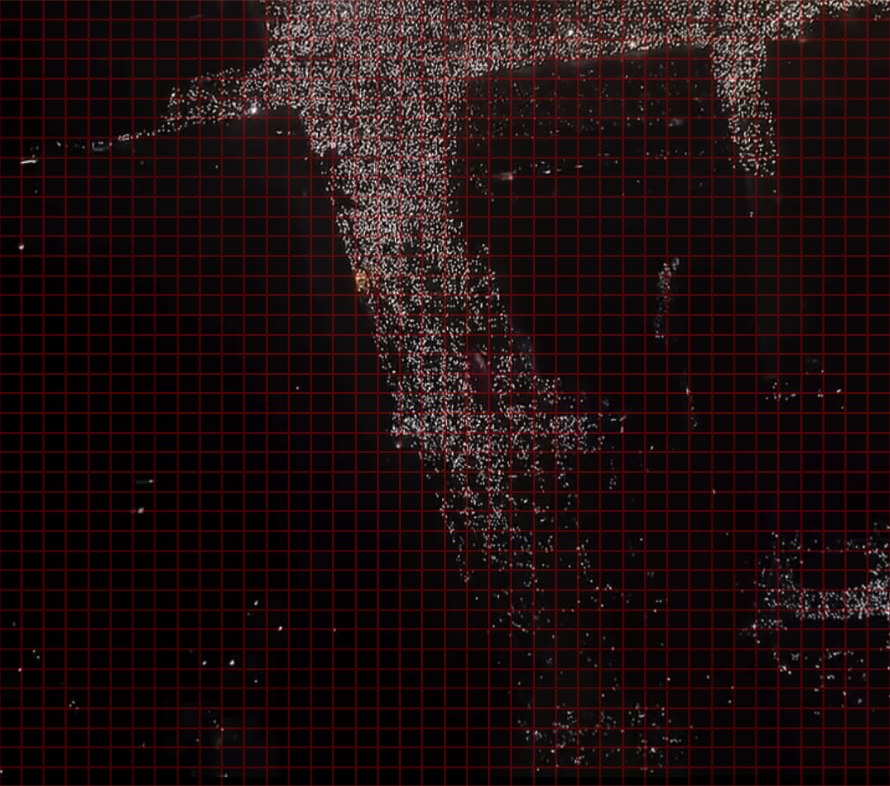
\includegraphics[width=\textwidth]{../grid_output/nemanjina_grid.png}
	  \caption{Nemanjina}
	  \label{fig:nemanjina}
	\end{subfigure}
	\hfill
	\begin{subfigure}[b]{0.3\textwidth}
		\centering
		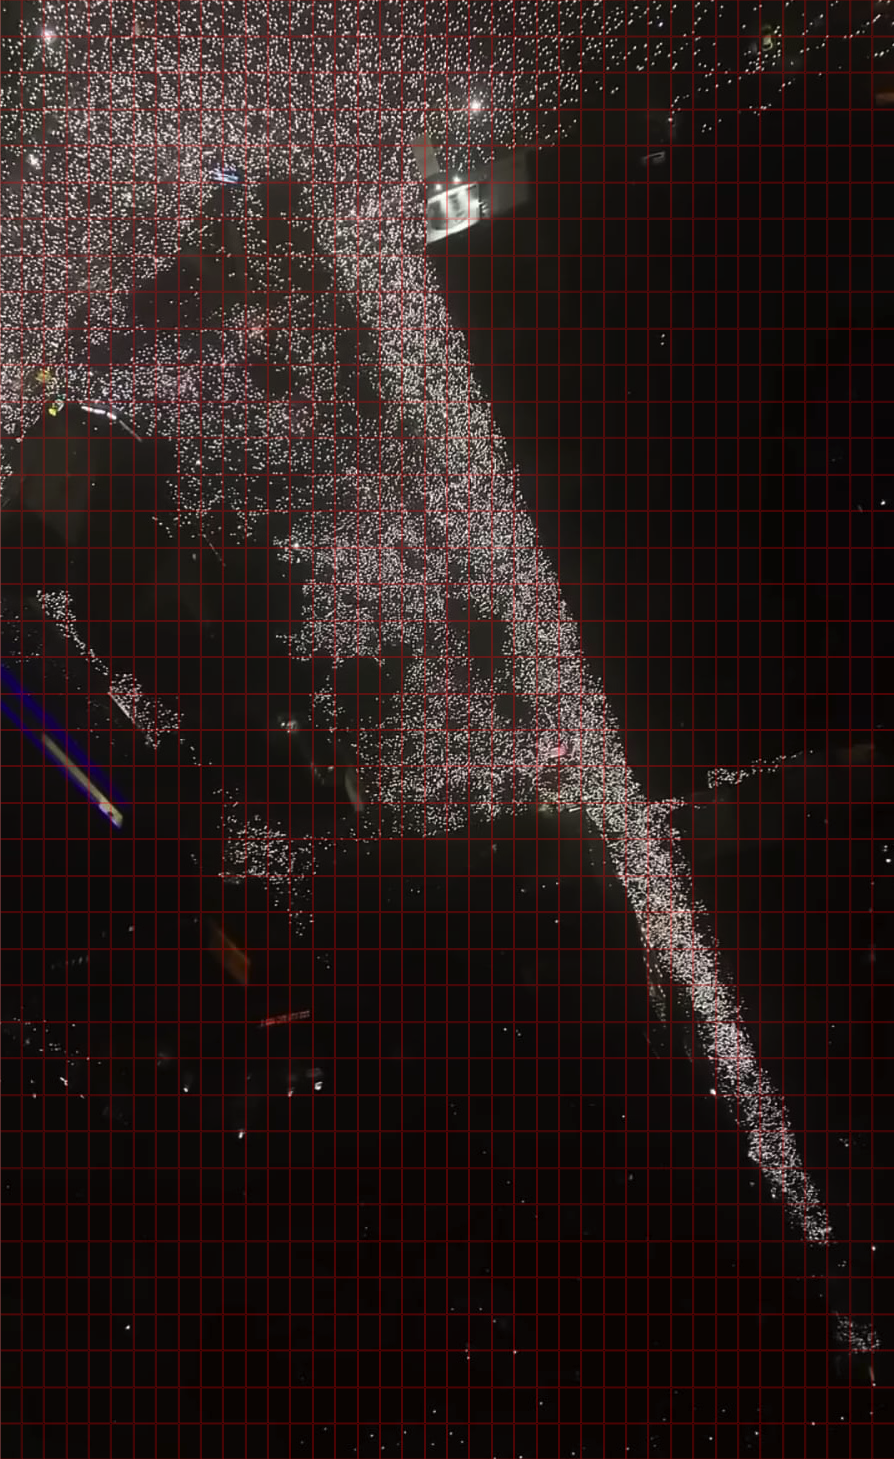
\includegraphics[width=\textwidth]{../grid_output/beogradska_grid.png}
		\caption{Beogradska}
		\label{fig:beogradska}
	\end{subfigure}
  
	\vspace{0.3cm} % razmak između redova
  
	% Drugi red
	\begin{subfigure}[b]{0.3\textwidth}
	  \centering
	  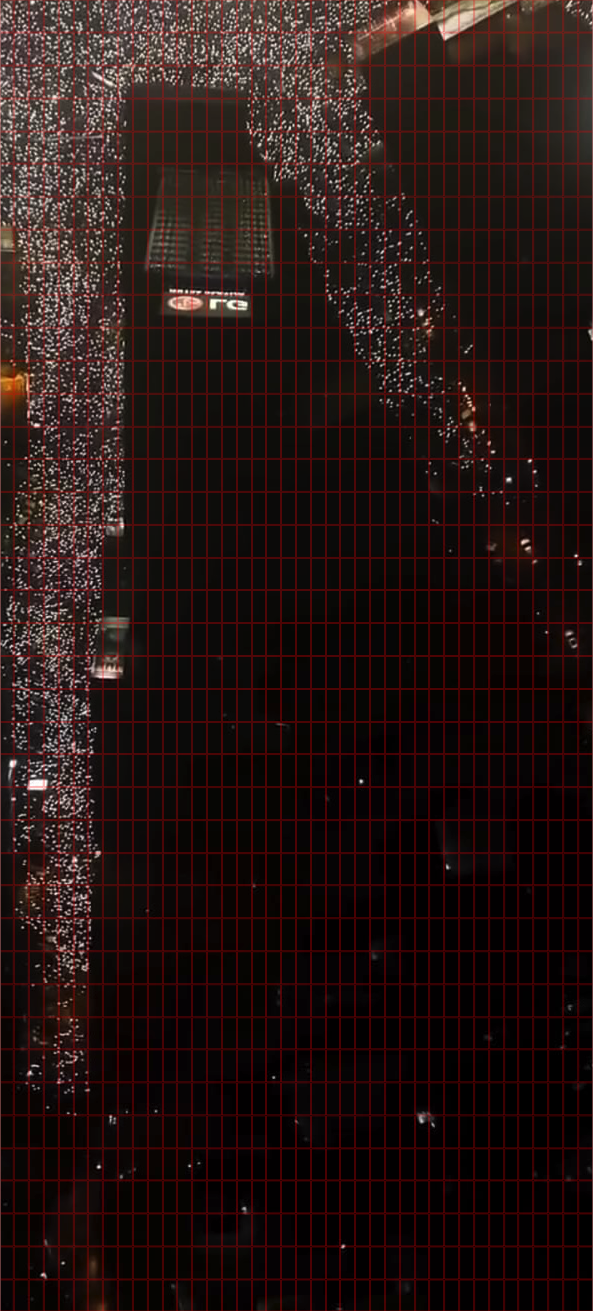
\includegraphics[width=\textwidth]{../grid_output/makenzijeva_grid.png}
	  \caption{Makenzijeva}
	  \label{fig:makenzijeva}
	\end{subfigure}
	\hfill
	\begin{subfigure}[b]{0.3\textwidth}
	  \centering
	  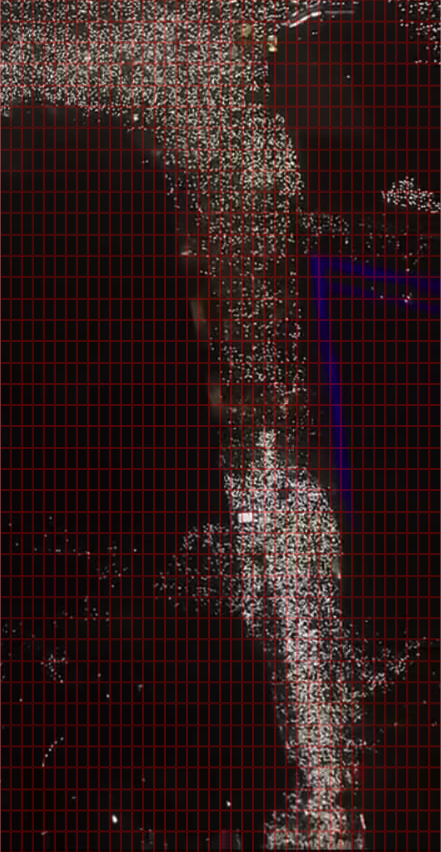
\includegraphics[width=\textwidth]{../grid_output/kralja-milana_grid.png}
	  \caption{Kralja Milana}
	  \label{fig:kralja-milana}
	\end{subfigure}
	\hfill
	\begin{subfigure}[b]{0.3\textwidth}
	  \centering
	  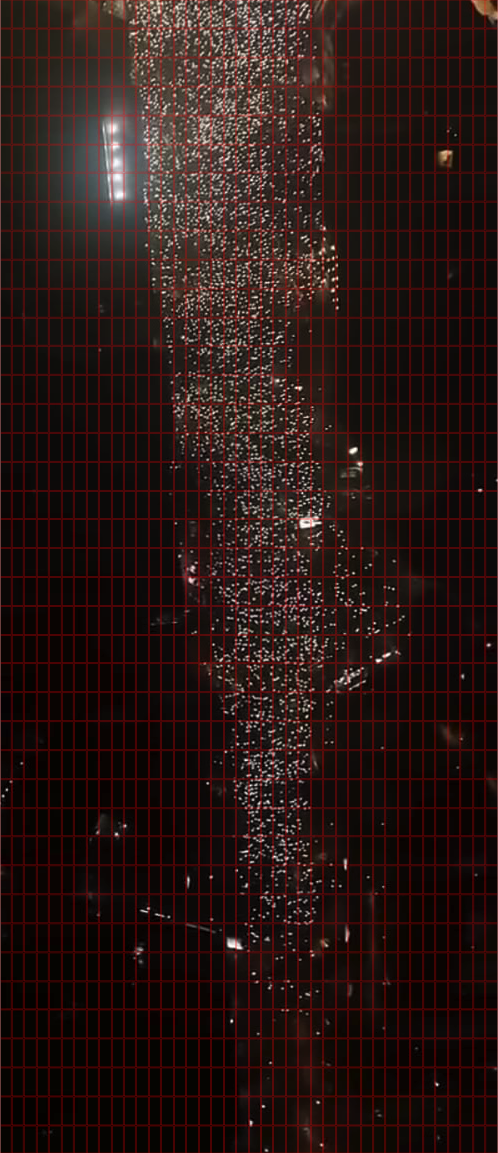
\includegraphics[width=\textwidth]{../grid_output/bulevar-oslobodjenja_grid.png}
	  \caption{Bulevar oslobođenja}
	  \label{fig:bulevar-oslobodjenja}
	\end{subfigure}
  
	\caption{Pregled ulica sa postavljenim grid-om}
\end{figure}

Radi smanjenja varijanse i troškova, uvodi se stratifikacija – grupisanje ćelija u tri stratuma (1 = najgušće, 2 = srednje, 3 = najređe).
Dodatno, gotovo „crne“ ćelije (bez informativnog sadržaja) sistematski se isključuju iz uzorkovanja.
\noindent
Dobijeni fajl \texttt{strata\_map\_auto.csv}, sa konačnim oznakama \texttt{include} i \texttt{stratum}, predstavlja osnovu za naredne korake – izbor pilot uzorka, primenu Neyman-ove alokacije i glavno uzorkovanje opisano u sledećim poglavljima, kao i za završnu procenu ukupnog broja ljudi.


\subsection{Automatska dodela stratuma (Python)}

Cilj je da automatski razvrstamo grid ćelije u 3 startuma po gustini i pouzdano isključimo neinformativne oblasti radi manjeg troška uzorkovanja i niže varijanse ocene.
Skripta \texttt{startum.py} za svaku ćeliju računa kompozitni skor gustine, koji kombinuje:
\begin{itemize}
    \item udeo svetlih piksela (\texttt{bright\_frac}),
    \item gustinu ivica (Canny edge detection),
    \item teksturnu varijansu (Laplacian variance).
\end{itemize}


\noindent Ulaz: \texttt{starta\_map.csv} (iz R grida) sa kolonama
\texttt{cell\_id, zone\_id, include, stratum, x0, x1, y0, y1, img\_path}.

\noindent Izlaz: \texttt{starta\_map\_auto.csv} — isto +
\texttt{strata\_score} (kompozitni skor), \texttt{black\_frac} (udeo “crnih” piksela), finalni include i stratum (1/2/3).
\newline
\newline
\noindent Ćelije kod kojih $ \ge 90\% $ piksela ima nisku osvetljenost (HSV V < 0.10) automatski se označavaju include = 0 i izuzimaju iz uzorkovanja. 
Preostale ćelije dele se na tri tercila po vrednosti kompozitnog skora: gornji tercil čini stratum 1, srednji stratum 2, a donji stratum 3.

\noindent
Automatska dodela se sastoji od sledećih koraka:
\begin{enumerate}
  \item \textbf{Maskiranje neinformativnih ćelija:} svaka ćelija se ispituje u HSV prostoru boja. Ako je udeo piksela sa niskom vrednošću osvetljenja (V) veći od zadatog praga (\texttt{black\_frac}, npr.\ 90\%), ćelija se automatski označava kao \texttt{include = 0}.
  \item \textbf{Računanje metrika:} za sve preostale ćelije izračunavaju se tri nezavisne metrike – udeo svetlih piksela (\texttt{bright\_frac}), gustina ivica (Canny edge detection) i teksturna varijansa (Laplacian variance).
  \item \textbf{Kombinovanje u kompozitni skor:} konačan \texttt{strata\_score} dobija se linearnom kombinacijom metrika sa težinama 0.4, 0.4 i 0.2.
  \item \textbf{Dodela stratuma:} ćelije sa \texttt{include = 1} dele se na tercile prema \texttt{strata\_score} (1 = gornji tercil, 2 = srednji, 3 = donji).
\end{enumerate}

\noindent
Najvažniji parametri skripte su prag za crnu boju \texttt{v\_black}, udeo crnih piksela \texttt{black\_frac}, prag za svetle piksele \texttt{v\_thresh}, prag zasićenja \texttt{s\_thresh}, kao i kvantil \texttt{low\_score\_q} za dodatno isključivanje najslabijih ćelija.

\subsection{Vizuelna provera stratuma (R)}

Rezultati automatske dodele vizuelizuju se, koja za svaku sliku prikazuje grid sa ćelijama obojenim po stratumu i zasenčenim poljima koja su isključena (include=0).
Crveno obojene su ćelije najveće gustine - startum = 1, žute su ćelije srednje gustine - stratum = 2, zelene ćelije najmanje gustine - startum = 3.
\newline
\noindent
Ovaj vizuelni korak služi kao brza kontrola kvaliteta: ukoliko se uoči da je algoritam označio kao gušće delove koji su u stvarnosti prazni (ili obrnuto), moguće je ručno prilagoditi vrednosti parametara i ponoviti automatsku dodelu.

\begin{figure}[H] 
	\centering 
	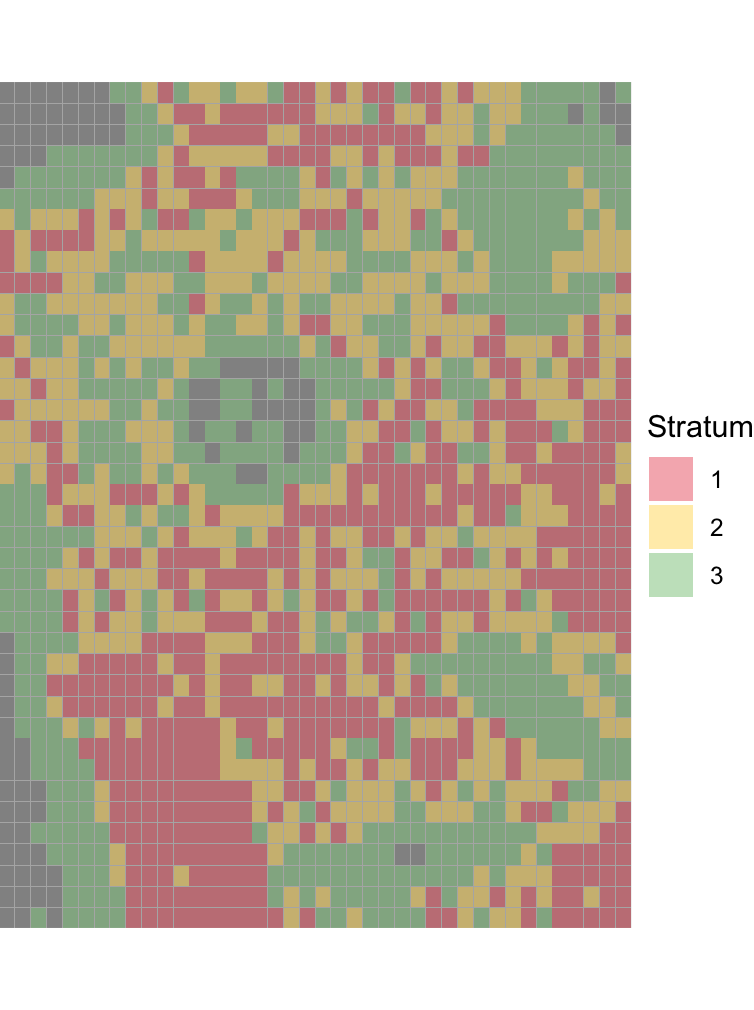
\includegraphics[width=0.8\textwidth]{../grid_output/strata_viz/slavija-centar_strata.png} 
	\caption{Slavija.} 
	\label{fig:slavija} 
\end{figure}

\begin{figure}[H]
	\centering
  
	% Prvi red
	\begin{subfigure}[b]{0.3\textwidth}
	  \centering
	  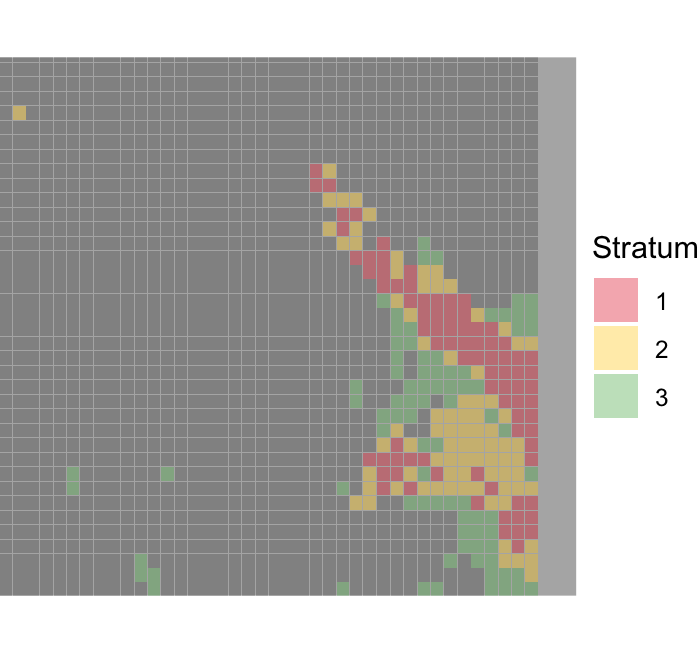
\includegraphics[width=\textwidth]{../grid_output/strata_viz/prote-mateje_strata.png}
	  \caption{Prote Mateje}
	  \label{fig:prote-mateje}
	\end{subfigure}
	\hfill
	\begin{subfigure}[b]{0.3\textwidth}
	  \centering
	  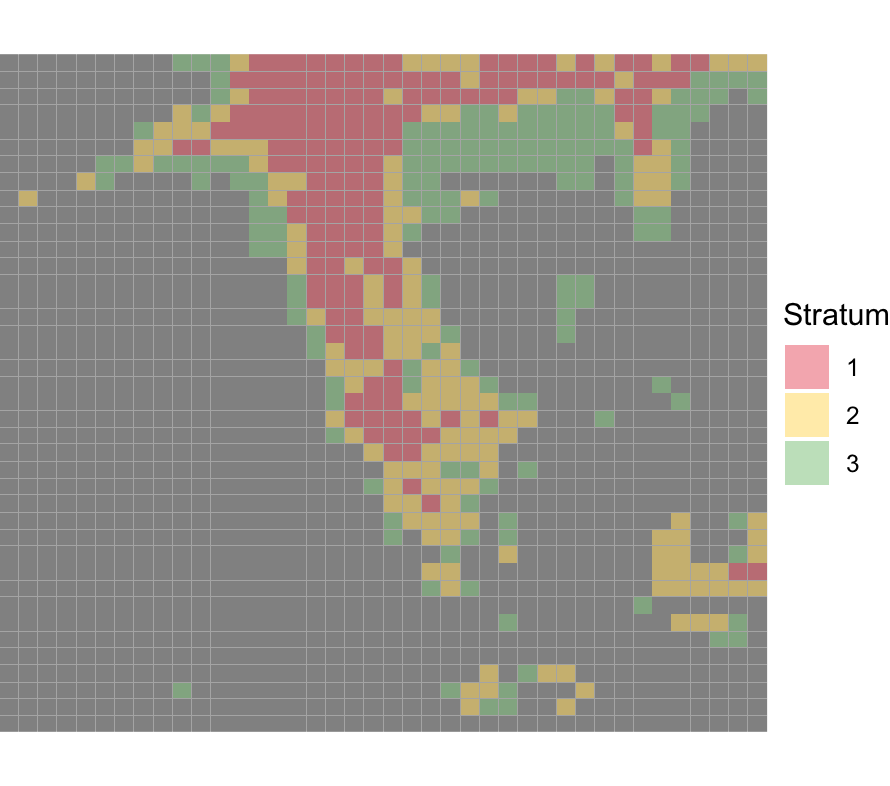
\includegraphics[width=\textwidth]{../grid_output/strata_viz/nemanjina_strata.png}
	  \caption{Nemanjina}
	  \label{fig:nemanjina}
	\end{subfigure}
	\hfill
	\begin{subfigure}[b]{0.3\textwidth}
		\centering
		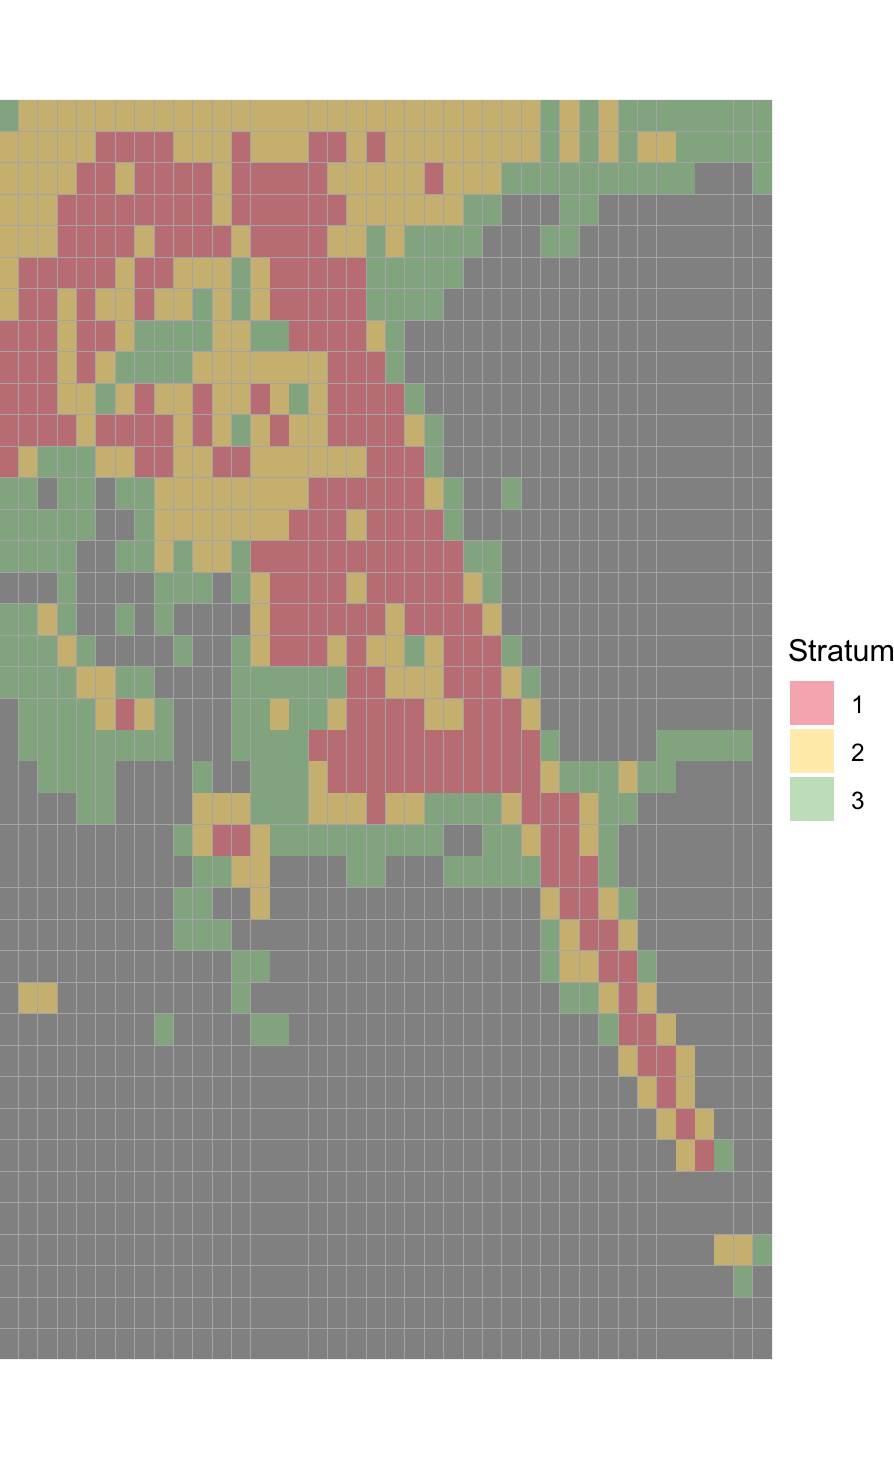
\includegraphics[width=\textwidth]{../grid_output/strata_viz/beogradska_strata.png}
		\caption{Beogradska}
		\label{fig:beogradska}
	\end{subfigure}
  
	\vspace{0.3cm} % razmak između redova
  
	% Drugi red
	\begin{subfigure}[b]{0.3\textwidth}
	  \centering
	  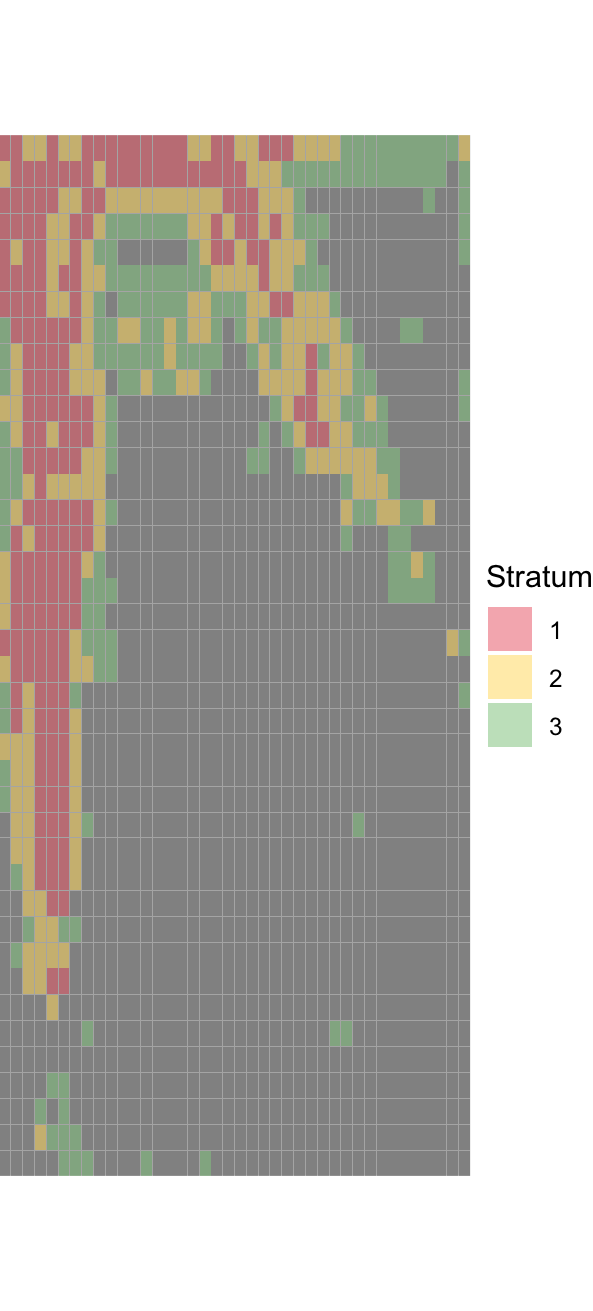
\includegraphics[width=\textwidth]{../grid_output/strata_viz/makenzijeva_strata.png}
	  \caption{Makenzijeva}
	  \label{fig:makenzijeva}
	\end{subfigure}
	\hfill
	\begin{subfigure}[b]{0.3\textwidth}
	  \centering
	  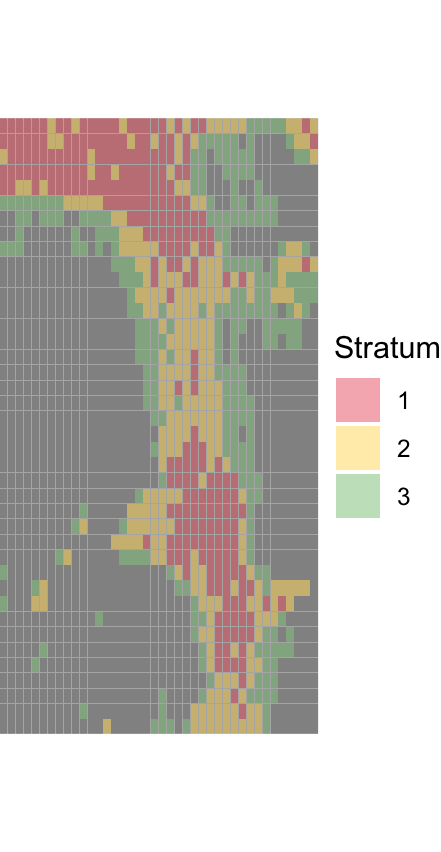
\includegraphics[width=\textwidth]{../grid_output/strata_viz/kralja-milana_strata.png}
	  \caption{Kralja Milana}
	  \label{fig:kralja-milana}
	\end{subfigure}
	\hfill
	\begin{subfigure}[b]{0.3\textwidth}
	  \centering
	  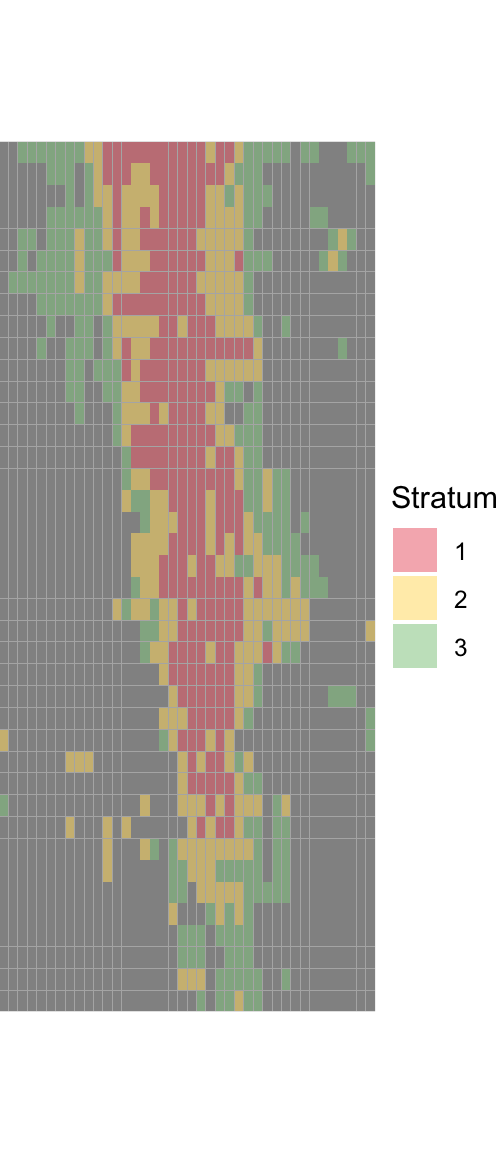
\includegraphics[width=\textwidth]{../grid_output/strata_viz/bulevar-oslobodjenja_strata.png}
	  \caption{Bulevar oslobođenja}
	  \label{fig:bulevar-oslobodjenja}
	\end{subfigure}
  
	\caption{Pregled ćelija po stratumima razlicitih gustina}
\end{figure}

\noindent
Nakon vizuelne provere i eventualnih korekcija, \texttt{strata\_map\_auto.csv} se koristi kao pouzdana ulazna baza za statističku analizu i uzorkovanje.

\section{Pilot uzorak i Neyman}

\section{Glavno uzorkovanje i brojanje “bliceva”}

\section{Procene i intervali poverenja}

\section{Rezultati i diskusija}

\section{Zaključak}


\newpage
\begin{thebibliography}{9}

	\bibitem{drone_video}
	Autor nepoznat. 
	\textit{Snimak javnog okupljanja dronom}. 
	Dostupno na: \url{https://youtube.com/shorts/4pbj2aZAoP4?si=wxzp9pIkflD2CYKN} 
	(Pristupljeno: 25. septembar 2025.)
	
	\end{thebibliography}

\end{document}